
% ----------------------------------------------------------------------
%  Set the document class
% ----------------------------------------------------------------------
\documentclass[11pt,a4paper,twoside]{article}

% ----------------------------------------------------------------------
% Define external packages, language, margins, fonts and new commands
% ----------------------------------------------------------------------
%\input{preamble} 
\usepackage[utf8]{inputenc}   % <<<<< Linux
\usepackage[english]{babel} % <<<<< English
\usepackage{notoccite}
\usepackage[skip=0.5\baselineskip]{caption}
\hyphenation{GTKWave}
\usepackage{listings}
\usepackage{amsmath, bm}
\usepackage[all]{nowidow}
\usepackage[table,xcdraw]{xcolor}

%blind text
\usepackage{lipsum}

\usepackage{graphicx}
\graphicspath{{./}{../../figlib/}{../mat/}{../sim/}}
\def\FontLn{% 16 pt normal
  \usefont{T1}{phv}{m}{n}\fontsize{16pt}{16pt}\selectfont}
\def\FontLb{% 16 pt bold
  \usefont{T1}{phv}{b}{n}\fontsize{16pt}{16pt}\selectfont}
\def\FontMn{% 14 pt normal
  \usefont{T1}{phv}{m}{n}\fontsize{14pt}{14pt}\selectfont}
\def\FontMb{% 14 pt bold
  \usefont{T1}{phv}{b}{n}\fontsize{14pt}{14pt}\selectfont}
\def\FontSn{% 12 pt normal
  \usefont{T1}{phv}{m}{n}\fontsize{12pt}{12pt}\selectfont}

% Use Arial font as default
%
\renewcommand{\rmdefault}{phv}
\renewcommand{\sfdefault}{phv}
\usepackage{geometry}	
\geometry{verbose,tmargin=2.5cm,bmargin=2.5cm,lmargin=2cm,rmargin=2cm}

%\usepackage{setspace}
%\renewcommand{\baselinestretch}{1.5}

\usepackage[pdftex]{hyperref} % enhance documents that are to be
                              % output as HTML and PDF
\hypersetup{colorlinks,       % color text of links and anchors,
                              % eliminates borders around links
%            linkcolor=red,    % color for normal internal links
            linkcolor=black,  % color for normal internal links
            anchorcolor=black,% color for anchor text
%            citecolor=green,  % color for bibliographical citations
            citecolor=black,  % color for bibliographical citations
%            filecolor=magenta,% color for URLs which open local files
            filecolor=black,  % color for URLs which open local files
%            menucolor=red,    % color for Acrobat menu items
            menucolor=black,  % color for Acrobat menu items
%            pagecolor=red,    % color for links to other pages
            pagecolor=black,  % color for links to other pages
%            urlcolor=cyan,    % color for linked URLs
            urlcolor=black,   % color for linked URLs
	          bookmarks=true,         % create PDF bookmarks
	          bookmarksopen=false,    % don't expand bookmarks
	          bookmarksnumbered=true, % number bookmarks
	          pdftitle={report},
            pdfauthor={Andre C. Marta},
%            pdfsubject={Thesis Title},
%            pdfkeywords={Thesis Keywords},
            pdfstartview=FitV,
            pdfdisplaydoctitle=true}

\usepackage[numbers,sort&compress]{natbib} % <<<<< References in numbered list [1],[2],...
\usepackage{subcaption} 
\usepackage{mdframed}

%%%%%%%%%%%%%%%%%%%%%%%%%%%%%%%%%%%%%%%%%%%%%%%%%%%%%%%%%%%%%%%%%%%%%%%%
%     Begin Document                                                   %
%%%%%%%%%%%%%%%%%%%%%%%%%%%%%%%%%%%%%%%%%%%%%%%%%%%%%%%%%%%%%%%%%%%%%%%%


\begin{document}

% Set plain page style (no headers, footer with centered page number)
\pagestyle{plain}

% Set roman numbering (i,ii,...) before the start of chapters
%\pagenumbering{roman}

% ----------------------------------------------------------------------
%  Cover page
% ----------------------------------------------------------------------
%%%%%%%%%%%%%%%%%%%%%%%%%%%%%%%%%%%%%%%%%%%%%%%%%%%%%%%%%%%%%%%%%%%%%%%%
%                                                                      %
%     File: Thesis_FrontCover.tex                                      %
%     Tex Master: Thesis.tex                                           %
%                                                                      %
%     Author: Andre C. Marta                                           %
%     Last modified :  2 Jul 2015                                      %
%                                                                      %
%%%%%%%%%%%%%%%%%%%%%%%%%%%%%%%%%%%%%%%%%%%%%%%%%%%%%%%%%%%%%%%%%%%%%%%%

\thispagestyle {empty}

% IST Logo - Signature A
% parameters: bb=llx lly urx ury (bounding box), width=h_length, height=v_length, angle=angle, scale=factor, clip=true/false, draft=true/false. 
\includegraphics[bb=9.5cm 11cm 0cm 0cm,scale=0.29]{IST_A_CMYK_POS}

\begin{center}
%
% Figure (Image or plot)
\vspace{1.0cm}
% height = 50 mm
%\includegraphics[height=50mm]{Figures/Airbus_A350.jpg}

% Title, author and degree
\vspace{1cm}
{\FontLb Circuit Theory and Electronics Fundamentals} \\ % <<<<< EDIT TITLE
\vspace{1cm}
{\FontSn Integrated Masters in Aerospace Engennering, Técnico, University of Lisbon} \\ % <<<<< EDIT COURSE
\vspace{1cm}
{\FontSn Laboratory Report 5- Bandpass Filter, Group 28} \\
\vspace{1cm}
{\FontSn Beatriz Pedroso 95773, Teresa Gonçalves 95826, Tiago Escalda 95851}\\
\vspace{1cm}
{\FontSn 6th June, 2021} \\ % <<<<< EDIT DATE (corresponds to date of oral examination)
%
\end{center}


\newpage

% ----------------------------------------------------------------------
% Dedication page (optional)
% ----------------------------------------------------------------------
%\input{dedication} 
%\cleardoublepage

% ----------------------------------------------------------------------
%  Acknowledgments (optional)
% ----------------------------------------------------------------------
%\input{acknowledgements}
%\cleardoublepage

% ----------------------------------------------------------------------
%  Abstract (both in English and Portuguese)
% ----------------------------------------------------------------------
%\input{resumo} 
%\cleardoublepage

%\input{abstract} 

% ----------------------------------------------------------------------
%  Table of contents, list of tables, list of figures and nomenclature
% ----------------------------------------------------------------------

% Table of contents
%
\tableofcontents
\newpage

% List of tables
%\addcontentsline{toc}{section}{\listtablename}
%\listoftables
%\cleardoublepage 

% List of figures
%\addcontentsline{toc}{section}{\listfigurename}
%\listoffigures
%\cleardoublepage 

% Set arabic numbering (1,2,...) after preface
%
%\setcounter{page}{1}
%\pagenumbering{arabic}

% ----------------------------------------------------------------------
%  Body
% ----------------------------------------------------------------------

\section{Introduction}
\label{introduction}


% state the learning objective
\par The aim of this laboratory assignment was to create an audio amplifier circuit. To do so, both the gain and the output stages were designed. This amplifier receives an audio maximum input of 10mV and connects to an 8 Ohm speaker. The source has an impedance of 100 Ohms and the circuit is supplied by a 12V Voltage DC source (vcc).
\par In the gain stage mentioned above, a NPN transistor and a common emitter amplifier with degeneration were used. It allows us to have a high $Z_{i}$ and a high $A_{V}$. Nevertheless, $Z_{o}$ is also very high, which consitutes a problem. Hence, this situation has to be adressed in the output stage. Consequently, in this second stage, it was used a common collecter amplifier and a PNP transistor. Not only does it allow to remain a high $A_{V}$ but it also reduces the value of $(Z_{o})$ significantly. Therefore, the gain is $\approx 1$, which is the desired result.

\par The quality of the audio amplifier is evaluated by the following expression:
\begin {equation}
	 MERIT = \frac{Voltage Gain*Bandwidth}{Cost*Lower Cut Off Frequency}   	
	\label{merit}
\end{equation}

The circuit is shown below.

\begin{figure}[ht] \centering
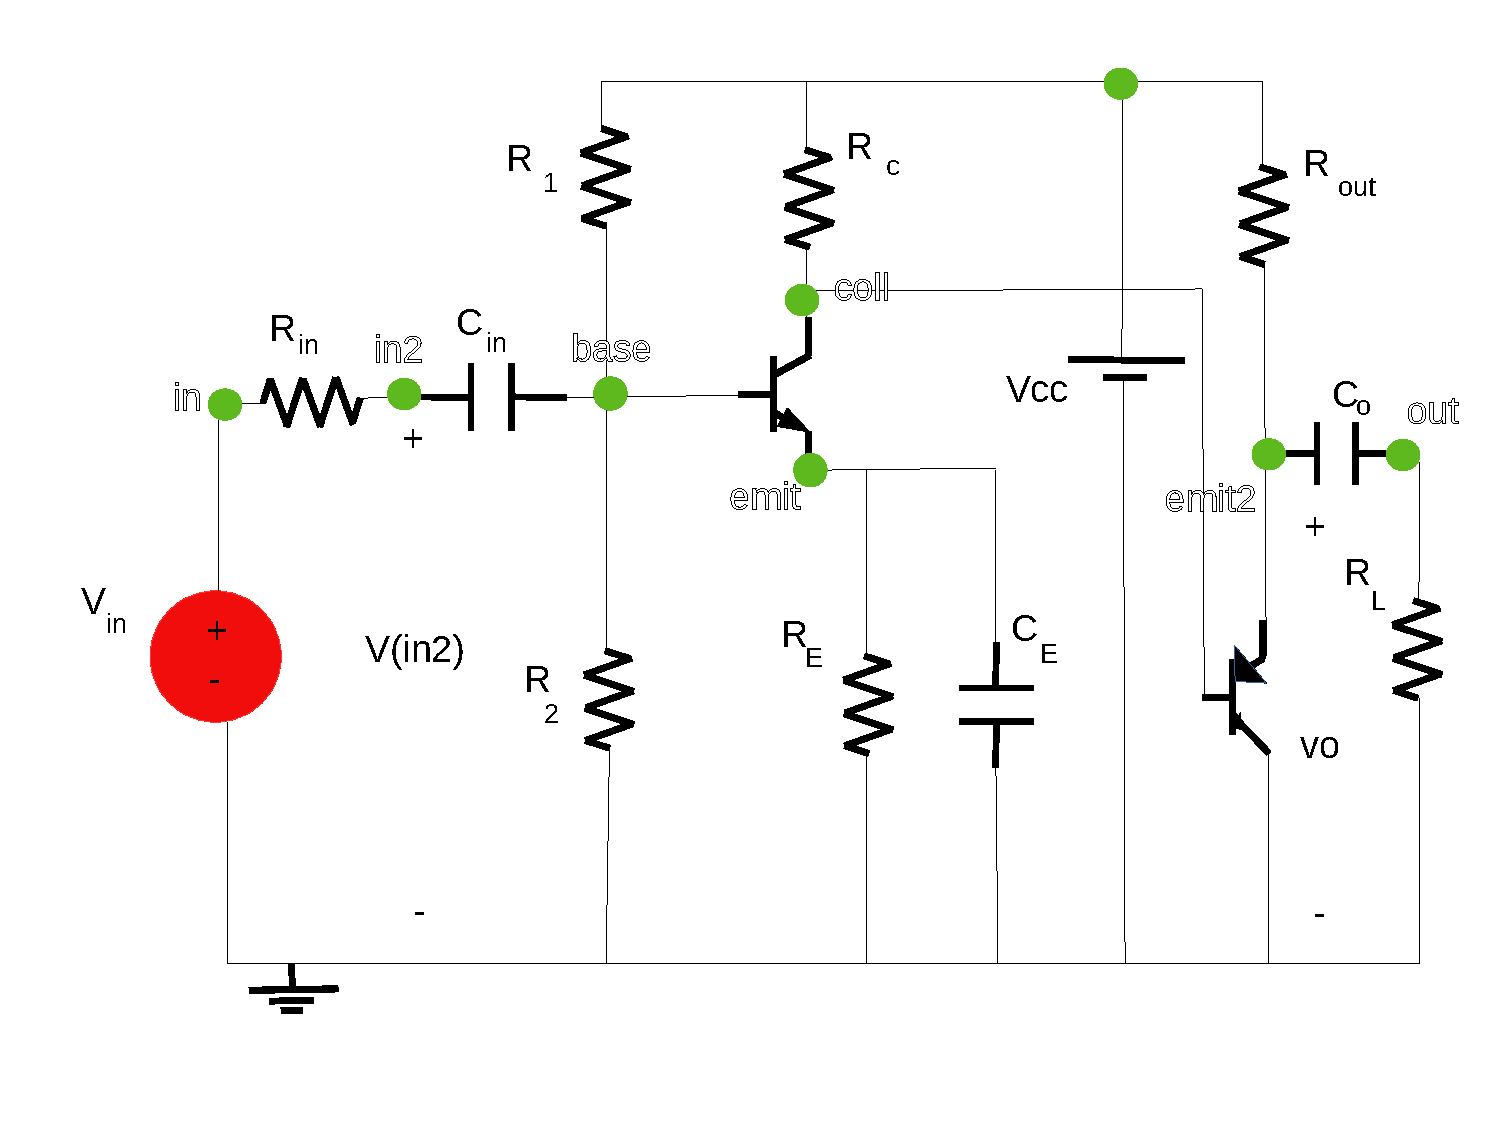
\includegraphics[width=0.8\linewidth]{lab4.pdf}
\caption{Circuit in analysis.}
\label{circuito todo}
\end{figure}


\newpage

\newpage

\section{Question 1- Nodal Analysis}


\subsection{Theoretical Analysis}




\subsection{Operating Point Analysis}
First of all, to contextualize the values obtained using the tools in ngspice, it is necessary to state that, as node 0 is connected to ground, its nodal voltage does not appear on the table of results. Furthermore, to be able to describe the voltage flowing in the dependent source, it is necessary to know the current in resistor 6. However, ngspice is not able to compute this value when the depedent source is described. So, in order to do that, an extra dependent voltage source (whose voltage drop is equal to 0 V) was created, and put in series after the resistor 6. This led to the appearence of node 8, that has the same voltage drop as node 6. So, by doing that, ngspice is able to determine the current in this auxiliar independent source, which is exactly the value needed.
 The circuit with these changes is shown in the drawing below.

\begin{figure}[ht] \centering
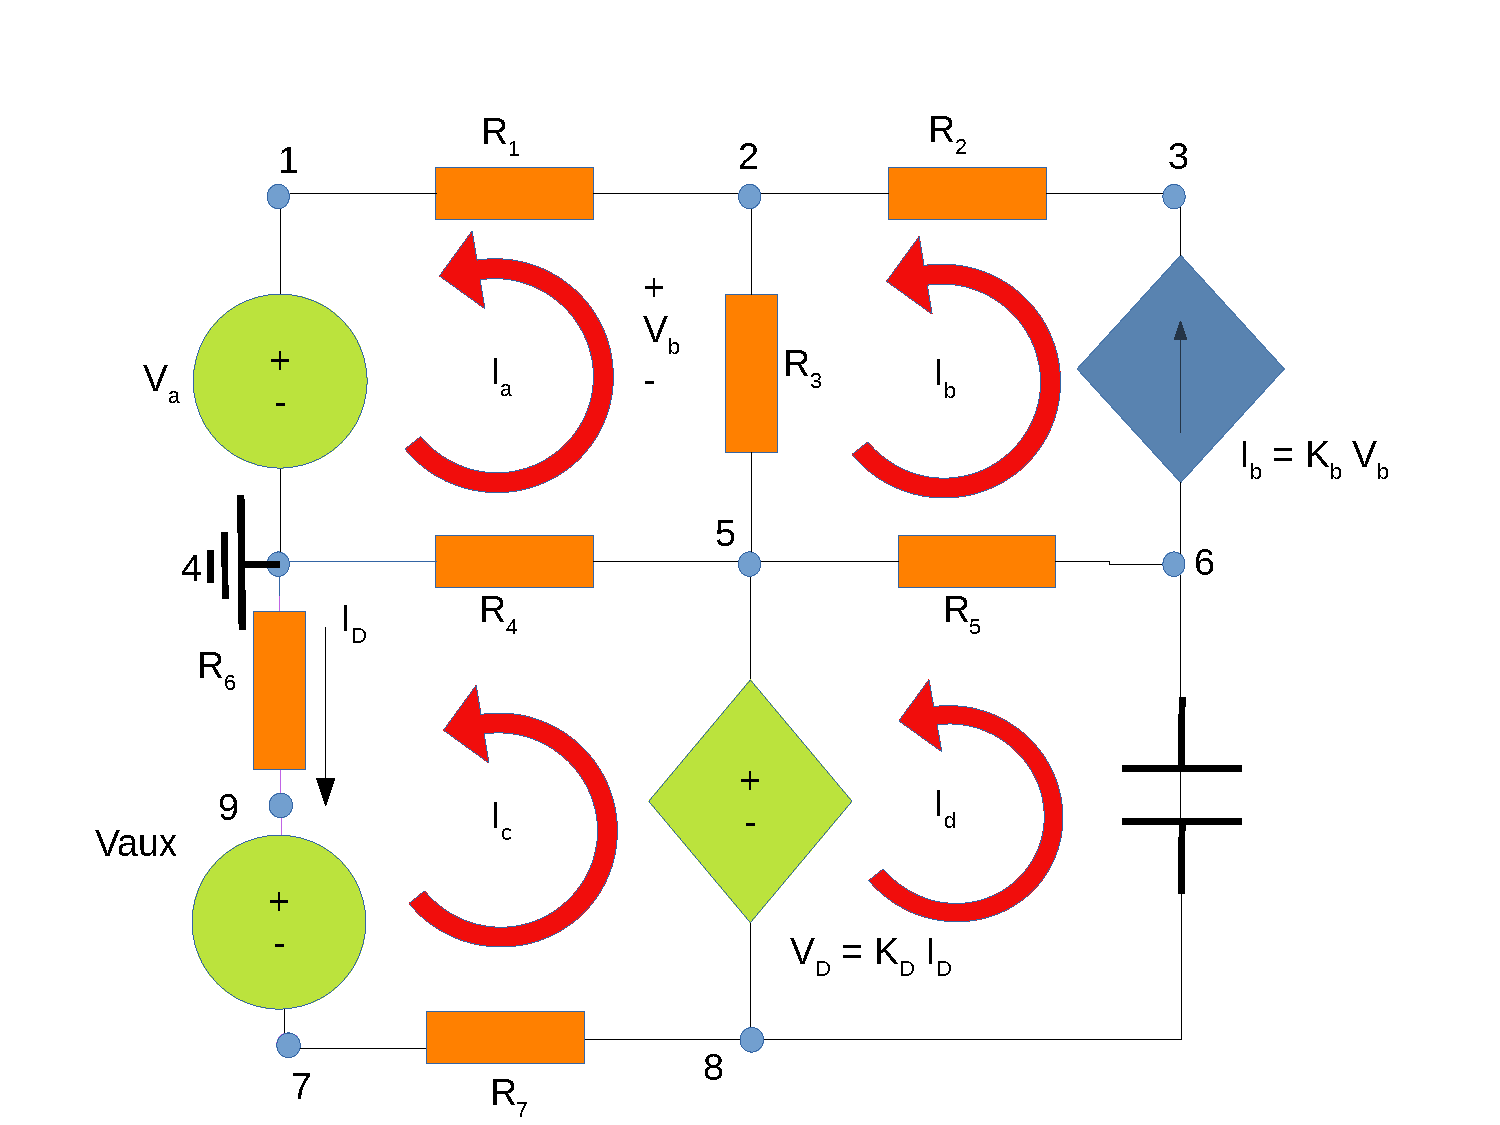
\includegraphics[width=1.0\linewidth]{sim1draw.pdf}
\caption{Circuit analysed in ngspice.}
\label{simdraw}
\end{figure}

\subsection{Comparison}
After running the simulation, the results were put in the table below. Then, a careful analysis of the aforementioned table was conducted.It shows the simulated operating point results for the circuit that is being studied, allowing the group to obtain the current flowing in every risistor, the voltage in the dependent voltage source and even the current flowing in the dependent currrent source. 

A variable preceded by @ is of type {\em current} and expressed in Ampere; other variables are of type {\it voltage} and expressed in
    Volt.
\begin{table}[ht]
\parbox{.45\linewidth}{
  \centering
  \begin{tabular}{|l|r|}
    \hline    
    {\bf Name} & {\bf Value [A or V]} \\ \hline
    @c1[i] & 0.000000e+00\\ \hline
@gb[i] & -2.26065e-04\\ \hline
@r1[i] & 2.161572e-04\\ \hline
@r2[i] & -2.26065e-04\\ \hline
@r3[i] & -9.90741e-06\\ \hline
@r4[i] & 1.183330e-03\\ \hline
@r5[i] & -2.26065e-04\\ \hline
@r6[i] & -9.67173e-04\\ \hline
@r7[i] & 9.671730e-04\\ \hline
v(1) & 5.068716e+00\\ \hline
v(2) & 4.843672e+00\\ \hline
v(3) & 4.369060e+00\\ \hline
v(5) & 4.874693e+00\\ \hline
v(6) & 5.579017e+00\\ \hline
v(7) & -1.98076e+00\\ \hline
v(8) & -2.97458e+00\\ \hline
v(9) & -1.98076e+00\\ \hline

  \end{tabular}
  \caption{Simulation and Calculus of Req (NgSpice)}} 
\parbox{.45\linewidth}{
  \centering
  \begin{tabular}{|l|r|}
    \hline    
    {\bf Name} & {\bf Value [A or V]} \\ \hline
    V1 & 5.068716e+00 \\ \hline
V2 & 4.843672e+00 \\ \hline
V3 & 4.369060e+00 \\ \hline
V4 & 0.000000e+00 \\ \hline
V5 & 4.874693e+00 \\ \hline
V6 & 5.579017e+00 \\ \hline
V7 & -1.980764e+00 \\ \hline
V8 & -2.974577e+00 \\ \hline

  \end{tabular}
  \caption{Simulation and Calculus of Req (NgSpice)}}
 
\end{table}


In order to validate the results obtained in NGSPICE, relative errors between the theoretical values, obtained in octave and the ones obtained in ngspice, were calculated. These were put in the table below.








\newpage

\section{Question 2- Nodal Analysis, and Req}
The purpose of this task was to compute the Req (equivalant resistance) of the circuit.

\subsection{Theoretical Analysis}
It is known that:
\begin{equation}
R_{eq}=\frac{V_{x}}{I_{x}}
\end{equation}
IN order to determine the variable aforementioned, first it was sugested to calculate it seen from the capacitors terminals. Then, using the Thevenin and Norton theorem, we put the independent voltage source to 0V. $V_{x}$ is equivalent to Thevenin's Voltage, and $I_{x}$ to Norton's Current. This is necessary because the depedent voltage short cannot be put equal to 0V(short-circuit) and the independent current source cannot be erased from the circuit.
\par An ilustration of the circuit analysed is showed in figure \ref{sim2draw} 
\begin{figure}[ht] \centering
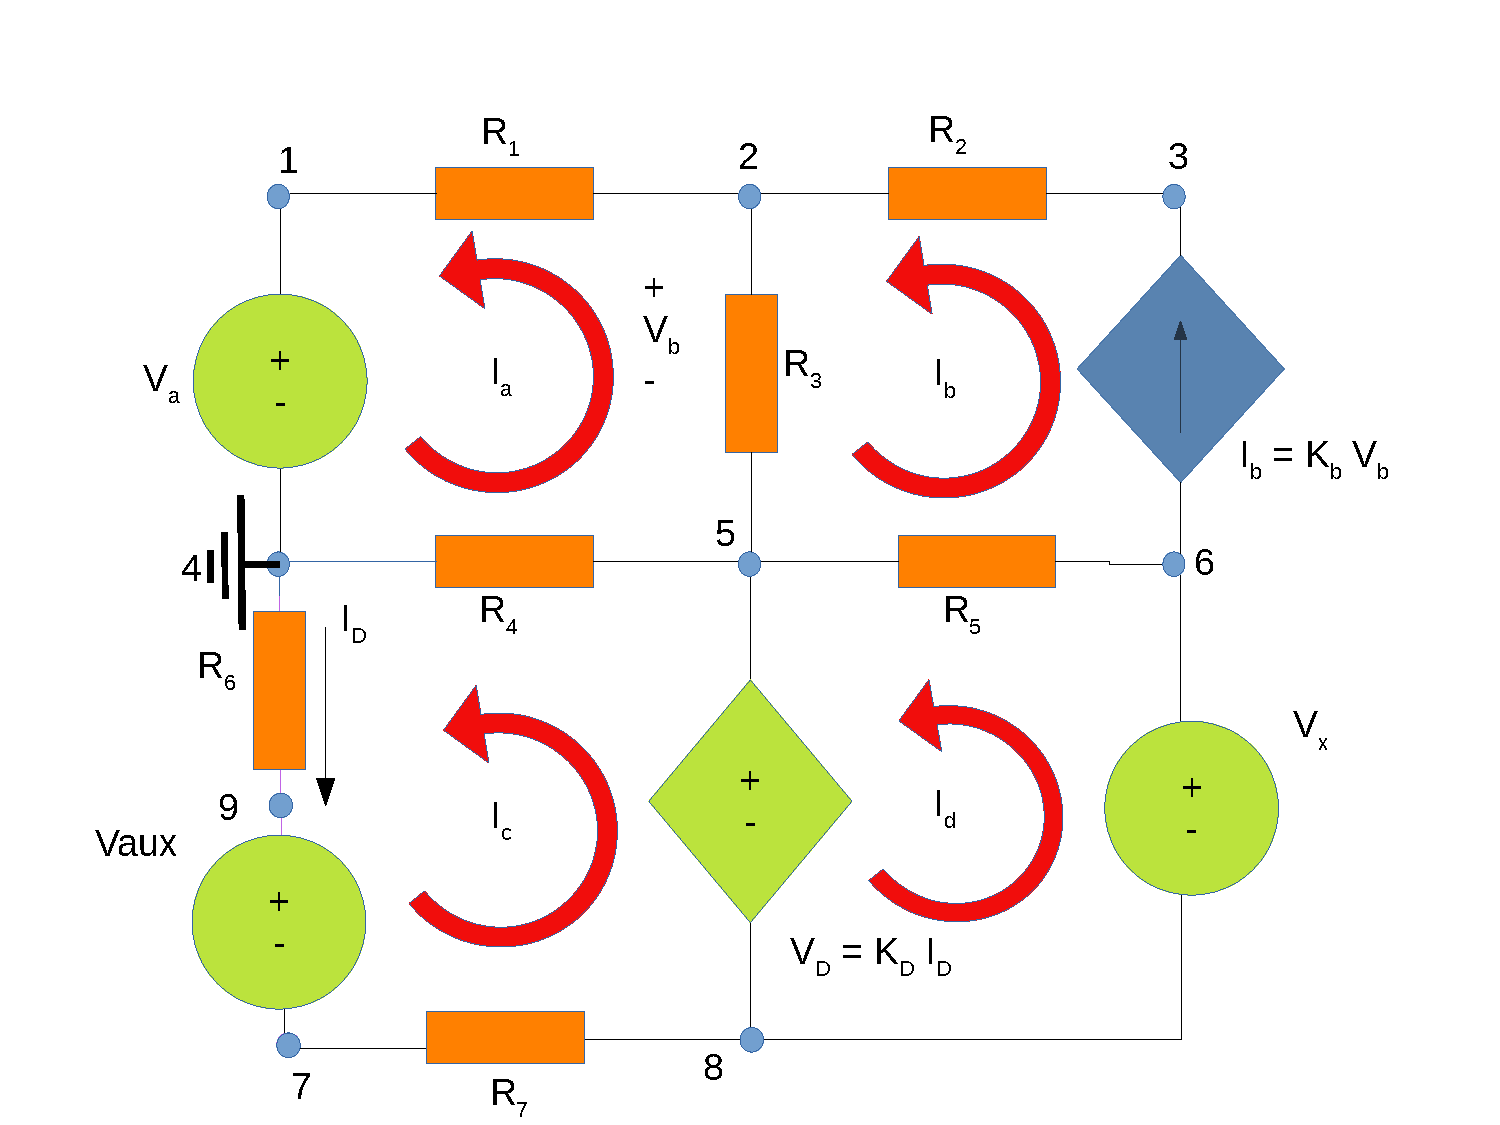
\includegraphics[width=1.0\linewidth]{sim2draw.pdf}
\caption{RC Circuit analysed in section 2.}
\label{sim2draw}
\end{figure}
\par
Then, the values of current of  every branch and the nodal values are obtained using node method. The matrix used in octave is the one that follows.

$\begin{bmatrix}
1 & 0 & 0 & 0 & 0 & 0 & 0 & 0 & 0\\
-G1 & G1+G2+G3 & -G2 & 0 & -G3 & 0 & 0 & 0 & 0\\
0 & -G2-Kb & G2 & 0 & Kb & 0 & 0 & 0 & 0\\
0 & 0 & 0 & 1 & 0 & 0 & 0 & 0 & 0\\
0 & -G1 & 0 & 0 & -G4 & 0 & -G6 & 0 & 0\\
0 & Kb & 0 & 0 & -G5-Kb & G5 & 0 & 0 & 1\\
0 & 0 & 0 & 0 & 0 & 0 & G6+G7& -G7 & 0\\
0 & 0 & 0 & 0 & 0 & 1 & 0 & -1 & 0\\
0 & 0 & 0 & KdG6 & -1 & 0 & -Kd*G6 & 1 & 0
\end{bmatrix}$
$\begin{bmatrix}
V1 \\ V2 \\ V3 \\ V4 \\ V5 \\ V6 \\ V7 \\ I_{x}
\end{bmatrix}$
= 
$\begin{bmatrix}
0 \\ 0 \\ 0 \\ 0 \\ 0 \\ 0 \\ 0 \\ V_{x} \\ 0
\end{bmatrix}$

\par Theoretically speaking, once the voltage source is equal to 0V, $V_{4}$ and  $V_{1}$ are also to be 0. 


\subsection{Operating Point Analysis}
As requested, an operating point analysis was conducted. The capacitor was replaced by the independent voltage source $V_{x}$ (\ref{sim2draw}). The values of currents and nodal voltages  were then put in a table, as well as the $R_{eq}$, hence:

\begin{equation}
R_{eq}=\frac{v(6)-v(8)}{vx#branch}}
\label{eq:4}
\end{equation}


\subsection{Comparison}
After running the node analysis in octave and the simulation in ngspice, the results were put in the tables below. Then, a careful analysis of the aforementioned tables was conducted.

A variable preceded by @ is of type {\em current} and expressed in Ampere; other variables are of type {\it voltage} and expressed in
    Volt. $R_{eq}$ is presented as in \ref{eq:4} in Ohm.

In order to validate the results obtained in NGSPICE, relative errors between the theoretical values, obtained in octave and the ones obtained in ngspice, were calculated. These were put in the table below.

\begin{table}[ht]
\parbox{.30\linewidth}{
  \centering
  \begin{tabular}{|l|r|}
    \hline    
    {\bf Name} & {\bf Value [A or V]} \\ \hline
    @c1[i] & 0.000000e+00\\ \hline
@gb[i] & 0.000000e+00\\ \hline
@r1[i] & 0.000000e+00\\ \hline
@r2[i] & 0.000000e+00\\ \hline
@r3[i] & 0.000000e+00\\ \hline
@r4[i] & 0.000000e+00\\ \hline
@r5[i] & 0.000000e+00\\ \hline
@r6[i] & 0.000000e+00\\ \hline
@r7[i] & 0.000000e+00\\ \hline
v(1) & 0.000000e+00\\ \hline
v(2) & 0.000000e+00\\ \hline
v(3) & 0.000000e+00\\ \hline
v(5) & 0.000000e+00\\ \hline
v(6) & 0.000000e+00\\ \hline
v(7) & 0.000000e+00\\ \hline
v(8) & 0.000000e+00\\ \hline
v(9) & 0.000000e+00\\ \hline

  \end{tabular}
  \caption{Simulation and Calculus of Req (NgSpice)}} 
\parbox{.30\linewidth}{
  \centering
  \begin{tabular}{|l|r|}
    \hline    
    {\bf Name} & {\bf Value [A or V]} \\ \hline
    V1 & 0.000000e+00 \\ \hline
V2 & 0.000000e+00 \\ \hline
V3 & 9.496396e-16 \\ \hline
V4 & 0.000000e+00 \\ \hline
V5 & 5.935248e-17 \\ \hline
V6 & 8.553593e+00 \\ \hline
V7 & -2.967624e-17 \\ \hline
V8 & 0.000000e+00 \\ \hline
Ix & -2.745419e-03 \\ \hline
Req & 3.115588e+03 \\ \hline
tau & 3.244185e-03 \\ \hline

  \end{tabular}
  \caption{Calculus of R_{eq}- Octave}}
 
\end{table}

\par After the careful evaluation of the results, several observations need to be made. Firstly, in ngspice, there are some node voltage results different from 0V, with  values  in the order of magnitude of 10^-15, 10^-16 V. After questioning the professor, these will be considered 0V.

\par On the other hand, octave results have equally those discrepancies. That said, the procedure was the same and those values were considered 0. We believe the main reason for this situation is that, when the data.txt file is read from the datagen.py in octave, a rounding happens, making it impossible for the nodal voltages to be 0. 

\par However, and despite the small erros above explaned, the values of $R_{eq}$, $V_{6}$ and $I_{x}$ match perfectly, which led us to fully validate the theorical procedure and the results obtained.




 


\newpage
\section{NATURAL RESPONSE}
It was proposed to study and determine the natural response of the circuit over time, in node 6. The natural response of the circuit is what the circuit does including the initial conditions (initial voltage of the capacitor) but with the imput supressed. 

\subsection{Theoretical Analysis}


In order to calculate the natural solution, we have to eliminate the voltage source, which means vs(t)=0V. Hence, we have an equivalent cicuit described by a voltage source and the capacitor. The current flowing through the capacitor is in fact consumed by it. Therefore, the voltage V8=0V and the amplitude Vx=V6-V8=V6.The natural solution will have the format $V{6n}(t)=A*e^{(-t/tau)}$ with tau=Req*C and A=V6 obtained in 2). As expected, the result is a negative exponencial graph, shown bellow.

\begin{figure}[ht] \centering
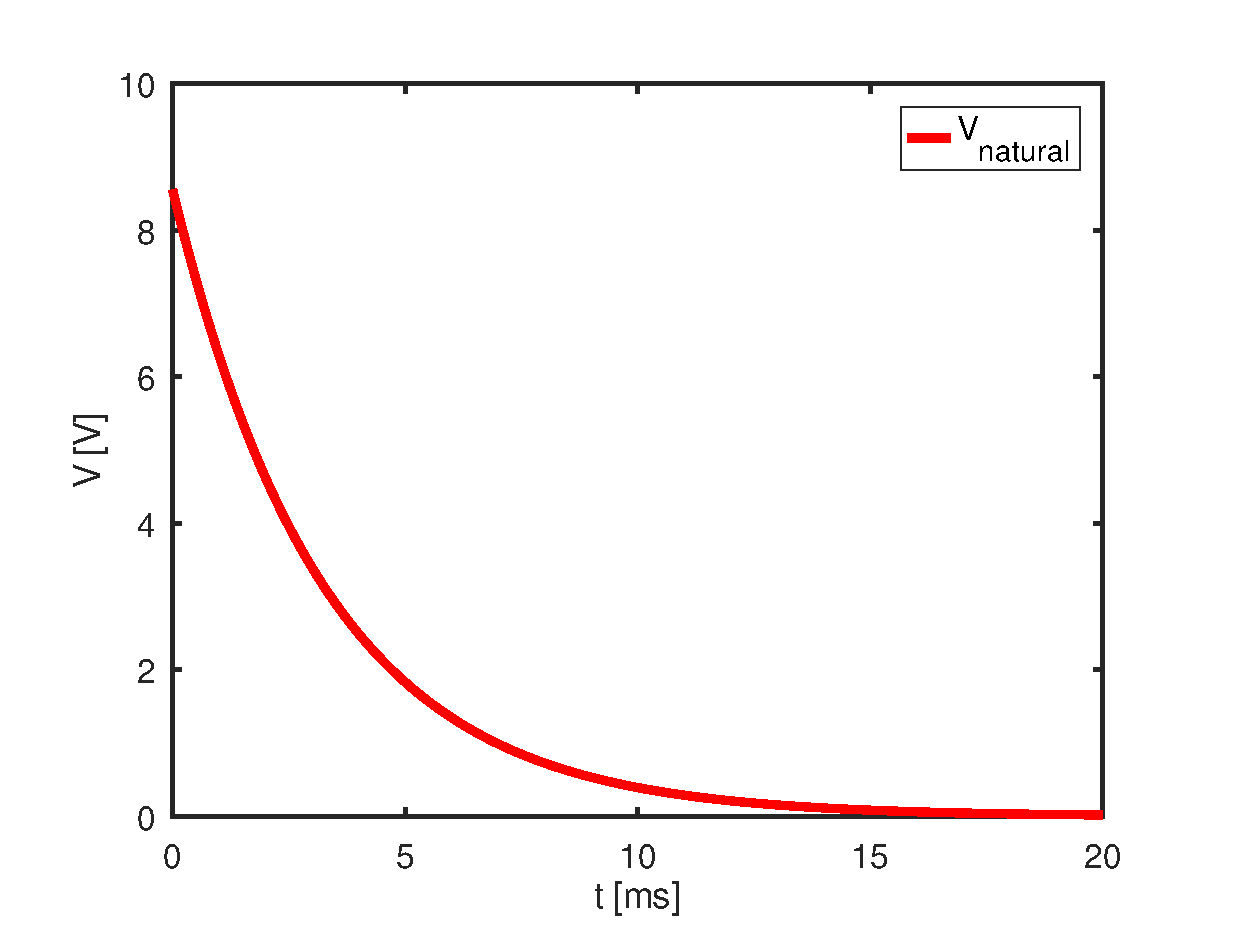
\includegraphics[width=0.5\linewidth]{natural.eps}
\caption{Circuit analysed.}
\label{fig:sim3}
\end{figure}


\subsection{Simulation Analysis}
In this section, a transient analysis was made in order to evaluate the natural response of the circuit, which means, the variation over time. The description of the circuit included the initial values of v(6) and v(8), calculated in question 1. As the ngspice and octave results matched, as observed in \ref{subsection:2.3}, the theorectical values were imported from a .cir file created by octave.
The time interval considered was [0,20]ms.
\begin{figure}[h] \centering
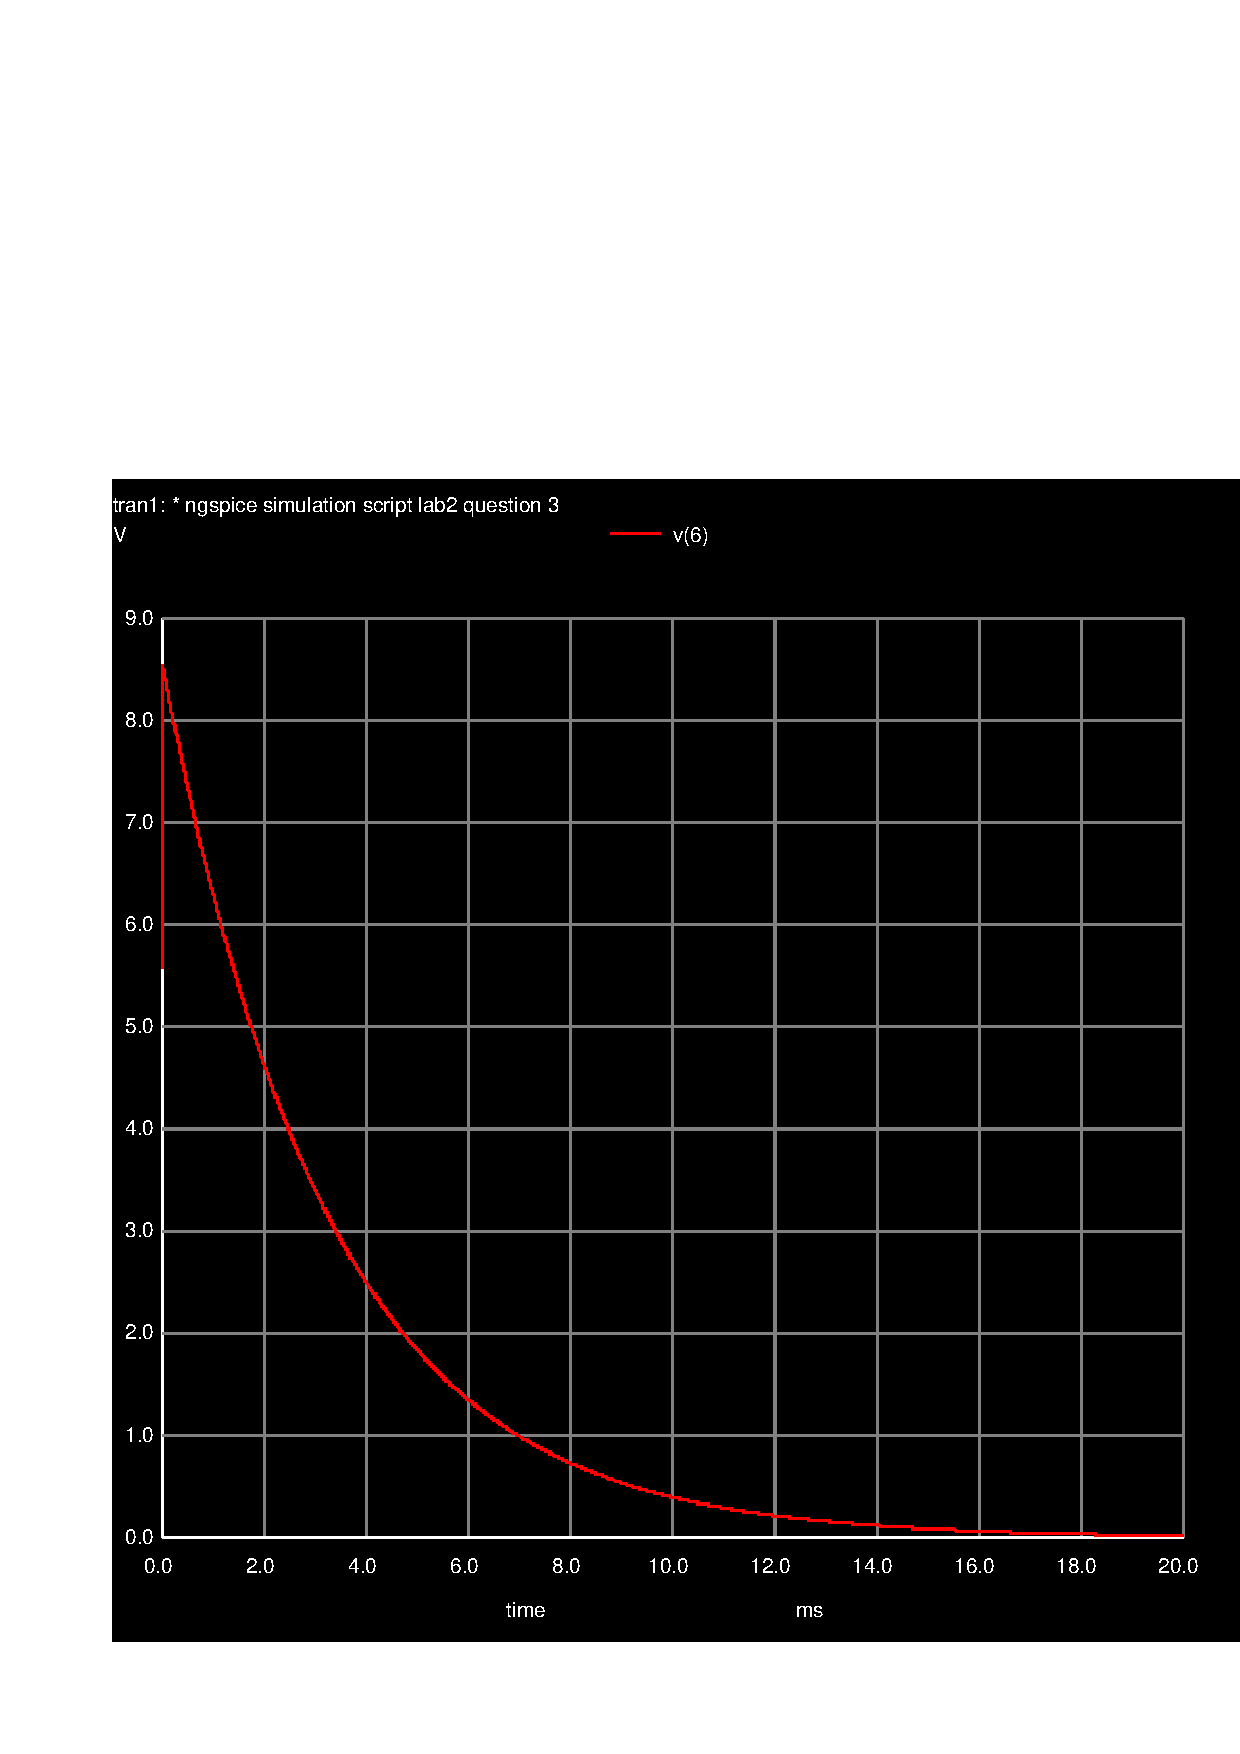
\includegraphics[width=0.5\linewidth]{sim3.pdf}
\caption{Circuit analysed.}
\label{fig:sim3}
\end{figure}
\newpage

\newpage
\section{Question 4- Theoretical Forced Response}
The forced response of a circuit is calculated with the sources turned on, but with the initial conditions (internal stored energy) set to zero.What is forced response? The forced response is where the output (the voltage on the capacitor) is going to end up in the long run after all stored energy eventually dissipates. The forced response does this by ignoring the presence of energy storage elements (in this case, it ignores the capacitor and its initial voltage). However, the forced response can't tell us what happens at t=0, or during the transition to the final state, because it ignores the stored energy. 
\par Like so, a phasor was used, with V_{s}=1. The capacitor was replaced by its impiedence $Z$. Then, the nodal method was run again, with this new variable.
\begin{equation}
w=2*pi*f
\end{equation} 

\begin{equation}
Zc=1/(j*w*C);
\end{equation} 

\par The matrix used was the following:

$\begin{bmatrix}
1 & 0 & 0 & -1 & 0 & 0 & 0 & 0 \\
-G1 & G1+G2+G3 & -G2 & 0 & -G3 & 0 & 0 & 0 \\
0 & -G2-Kb & G2 & 0 & Kb & 0 & 0 & 0 \\
0 & 0 & 0 & 1 & 0 & 0 & 0 & 0 \\
0 & G3 & 0 & G4 &-G3-G5-G4 & G5+1/Zc & G7 & -G7-1/Zc\\
0 & Kb & 0 & 0 & -G5-Kb & G5+1/Z_{c} & 0 & -1/Z_{c} \\
0 & 0 & 0 & 0 & 0 & 0 & G6+G7& -G7 \\
0 & 0 & 0 & KdG6 & -1 & 0 & -Kd*G6 & 1
\end{bmatrix}$
$\begin{bmatrix}
V1 \\ V2 \\ V3 \\ V4 \\ V5 \\ V6 \\ V7 \\ 
\end{bmatrix}$
= 
$\begin{bmatrix}
1 \\ 0 \\ 0 \\ 0 \\ 0 \\ 0 \\ 0 \\ 0 \\ 
\end{bmatrix}$

\par Then, the complex amplitudes with the knowlegde that the amplitude of the forced response is the absolute value of the complex $V_{6}$ (\Alpha), and the phase(\Theta) is the argument, the forced solution is then given by:

\begin{equation}
V6_f=\Alpha*sin(w*t+\Theta)
\end{equation} 

\par The table below presents the values of the complex amplitudes of every nodal voltage:

begin{table}[ht]
{
  \centering
  \begin{tabular}{|l|r|}
    \hline    
    {\bf Name} & {\bf Value [V]} \\ \hline
    V1 & 1.000000e+00 \\ \hline
V2 & 9.556014e-01 \\ \hline
V3 & 8.619659e-01 \\ \hline
V4 & 2.801649e-17 \\ \hline
V5 & 9.617215e-01 \\ \hline
V6 & 5.886212e-01 \\ \hline
V7 & 3.907822e-01 \\ \hline
V8 & 5.868501e-01 \\ \hline

  \end{tabular}
  \caption{Amplitudes of Nodal Voltages} 
\end{table}





\newpage
\section{Question 5 (Theorectial) and 4 (Simulation)-Natural and Forced Response}

The total response of a circuit can be teased apart into a forced response plus a natural response. These responses can be combined using the principle of superposition. This principle pressupose the addition of the natural response and the forced response, both calculated in question 3 and 4.

\subsection{Theoretical Analysis}

\begin{figure}[ht] \centering
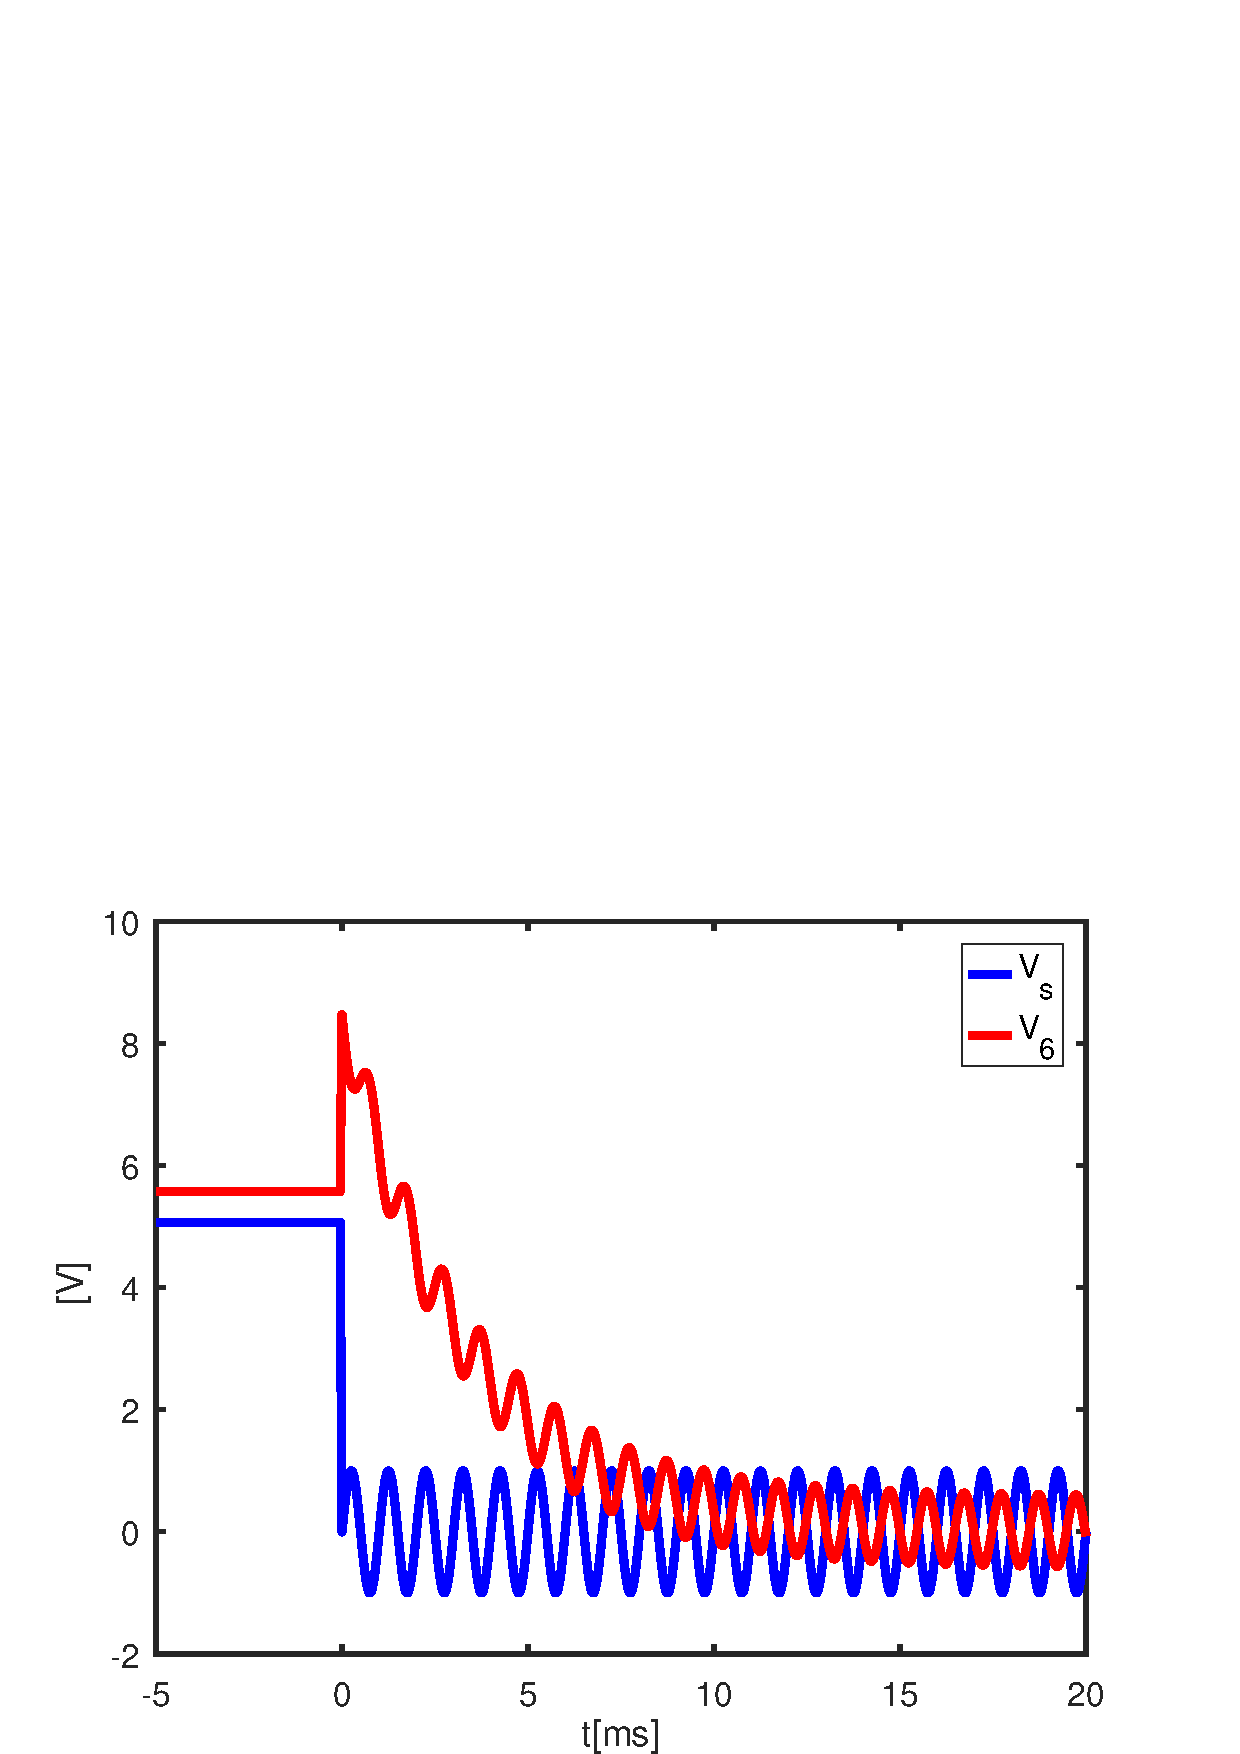
\includegraphics[width=0.9\linewidth]{part4.pdf}
\caption{Circuit analysed.}
\label{fig:sim4}
\end{figure}



\subsection{Simulation Analysis}
Once again, a transient analysis was made in order to meet the goal above. The main difference between the analysis in point 3 and this one is that Vs was considered a sinusoidal voltage source. This way, the plot obtained is the sum of both responses.

\begin{figure}[ht] \centering
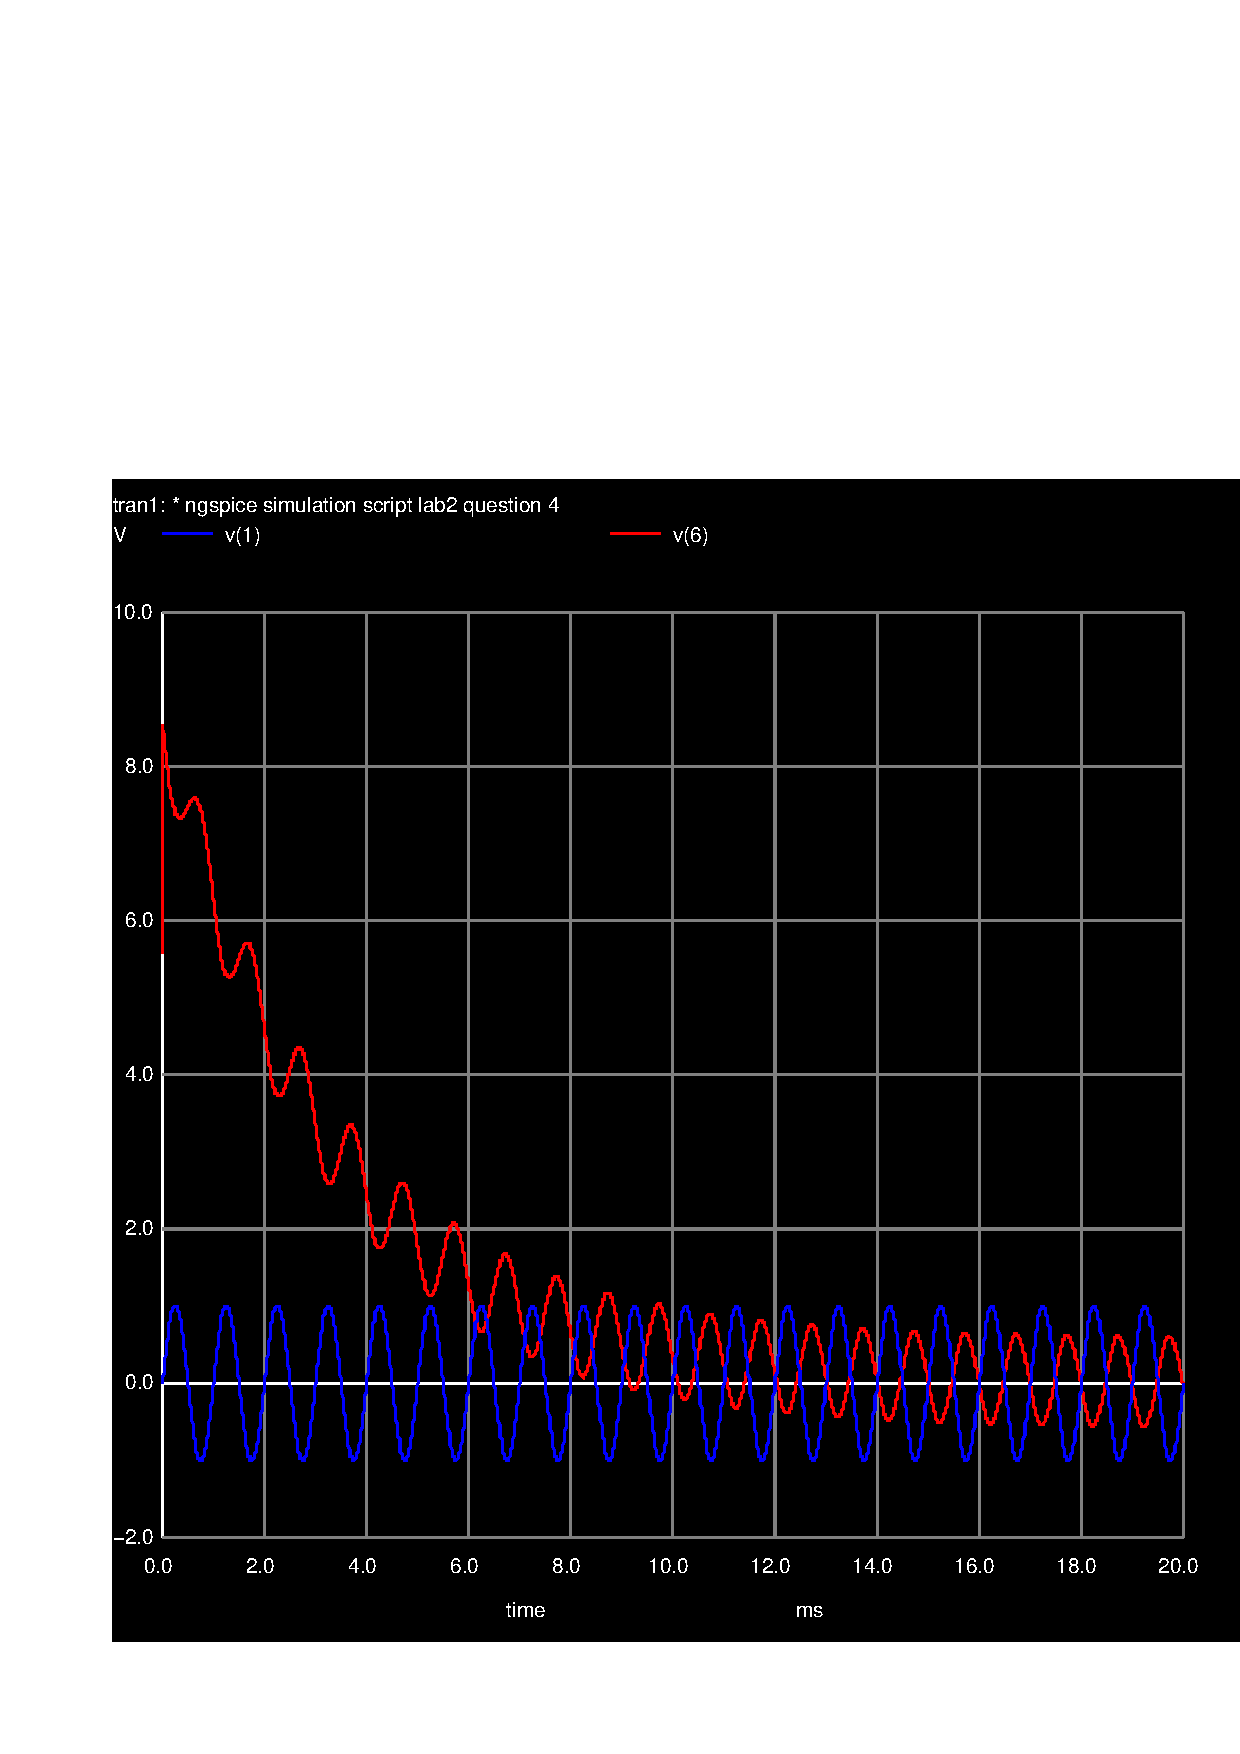
\includegraphics[width=0.9\linewidth]{sim4.pdf}
\caption{Circuit analysed.}
\label{fig:sim4}
\end{figure}

\subsection{Comparison}


\newpage
\section{Question 6 (Theoretial) and 5 (Simulation)-Frequency Response}
In this section, both octave and ngspice were used in order to obtain plots of the phase response and of the magnitude response, using logscale. This approach is very useful hence it provides a much better plot fit and, therefore it provides great visualization for users. The magnitude in debicels is of interest for analysis of sound waves, and the analysis of the phase or angle delay is a very interesting way of study another parameter to compare signal. Frequency range in both analysis was from 0.1 Hz to 1MHz. The plots made were v6(f), vs(f) and vc=(v6(f)-v8(f)).

\subsection{Theoretical Analysis}

To examine the frequency responses, the system of equations in Section 4 is solved in a loop cycle, what allows us to calculate the $V_6$, $V_c$ and $V_s$ for each frequence. For each result of these complex vectors, the values were saved.

\subsubsection{Frequency Response- Magnitude}

To represent the magnitude in dB, the absolute values were converted ($X_{dB}$=20$log_{10}$(X)). The frequencies were put in a logarithmic scale.

The magnitude of $V_s$ does not suffer any alteration with the variation of the frequency of the signal. Since its amplitude is 1, as one can observe in the graphics shown at the end of the section, the plot shows a constant horizontal line, with the value zero (0=$log_{10}$(1)).

On the contrary, as the frequency is increasing, the magnitudes of $V_6$ and $V_c$ decrease. The value of $V_c$ changes as it is expected in a RC circuit. This is due to the impedance of the capacitor (Z=-j/wC).

\subsubsection{Frequency Response- Phase}


The angles of the values saved were transformed from radians to degrees. The phase in $V_s$ is 0, therefore we do not have to do any further calculations. The phase of each voltage corresponds to the exact angles. In the plot shown below, the frequencies were also  put in the logarithmic scale. As the frequency increases the phase tend to negative values, which varies as it is expected.


\subsection{Simulation Analysis}
In this part of the assignment, an AC (Small Signal Analysis was conducted, in order to match the goal aforementioned. This type of analysis allows to study the frequency response of the circuit. In other words, there is no frequency variation over time, the so called steady-state analysis.

\subsection{Comparison}
After comparing the graphics showed below, it is clear to admit that the results in ngspice and octave match. Any minor difference may be explained by aproximation errors.

\subsubsection{Frequency Response- Magnitude}


\begin{figure}[ht] \centering
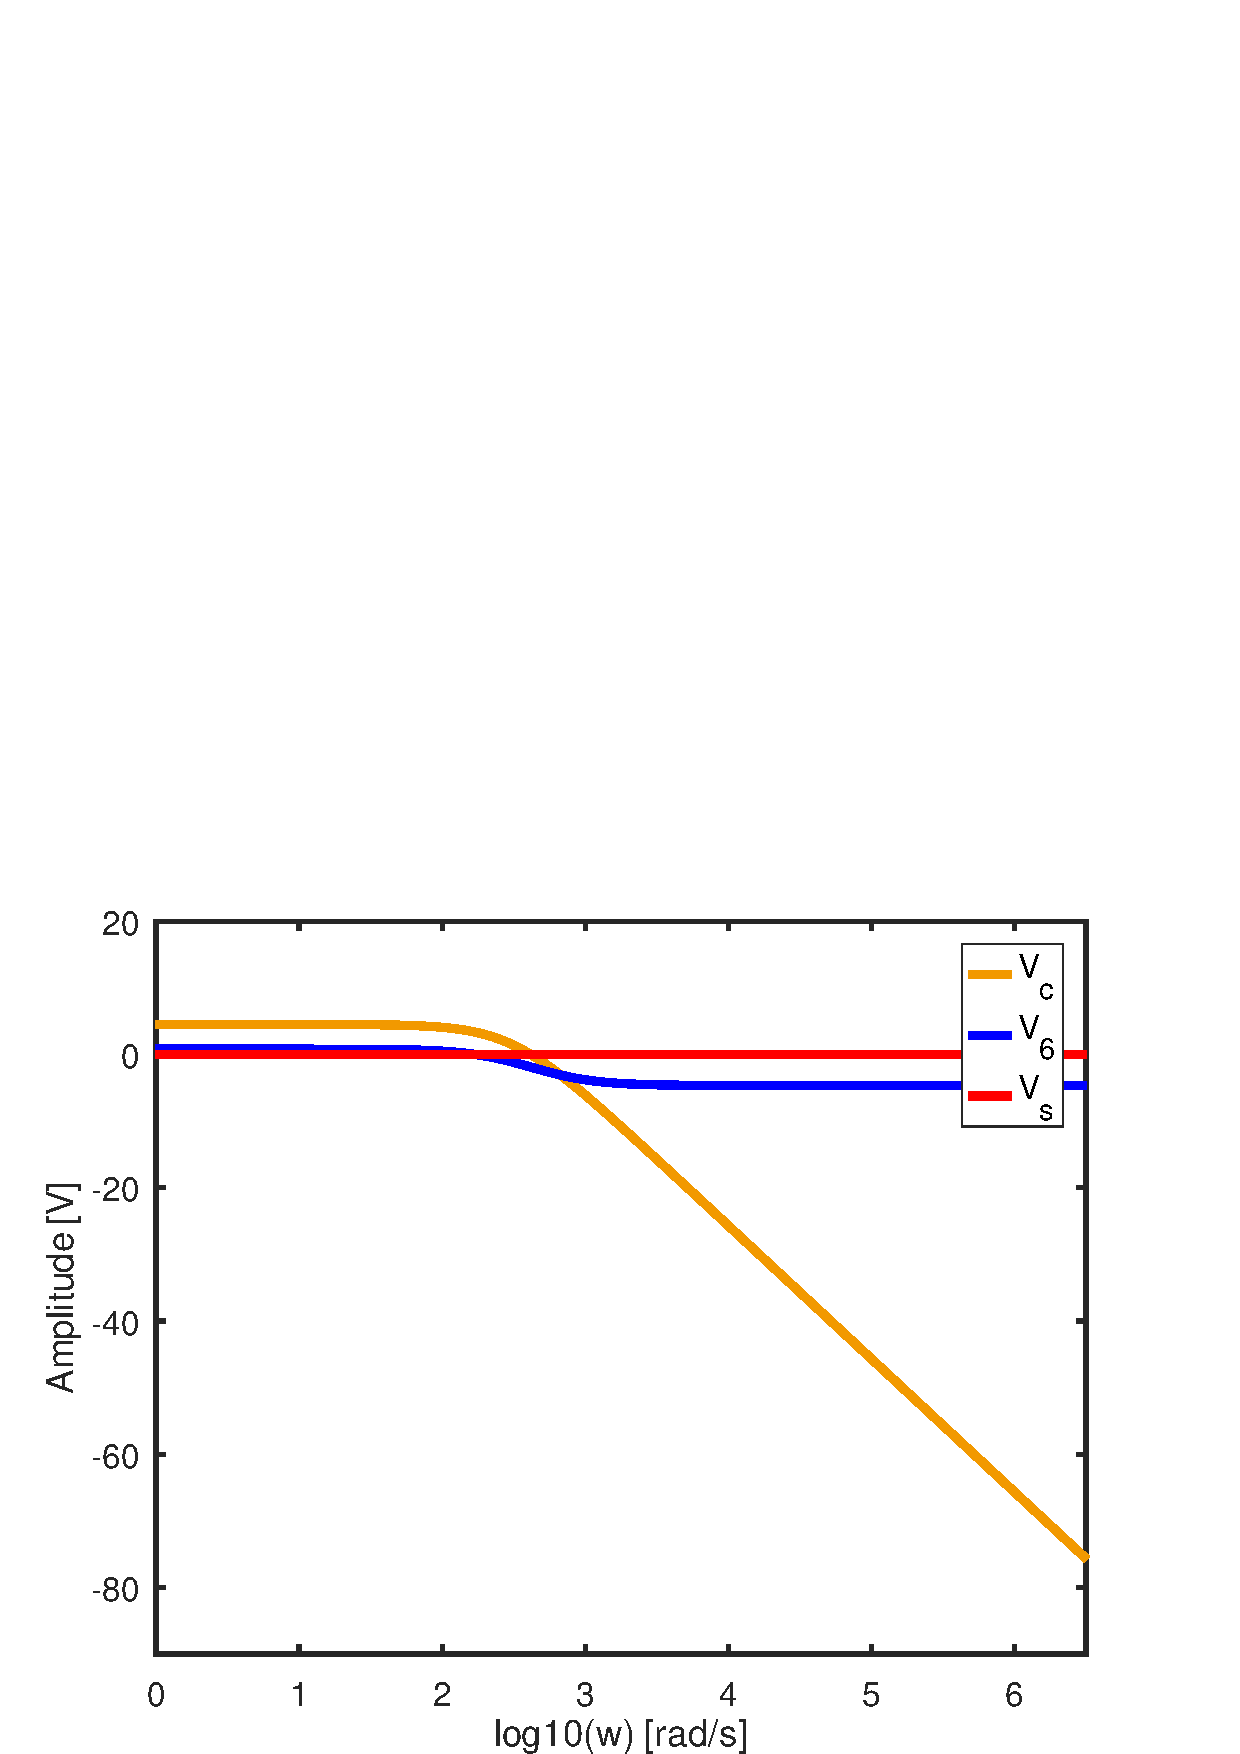
\includegraphics[width=0.9\linewidth]{part6_amp.pdf}
\caption{Circuit analysed.}
\label{RC Circuit.}
\end{figure}


%\begin{figure}[ht] \centering
%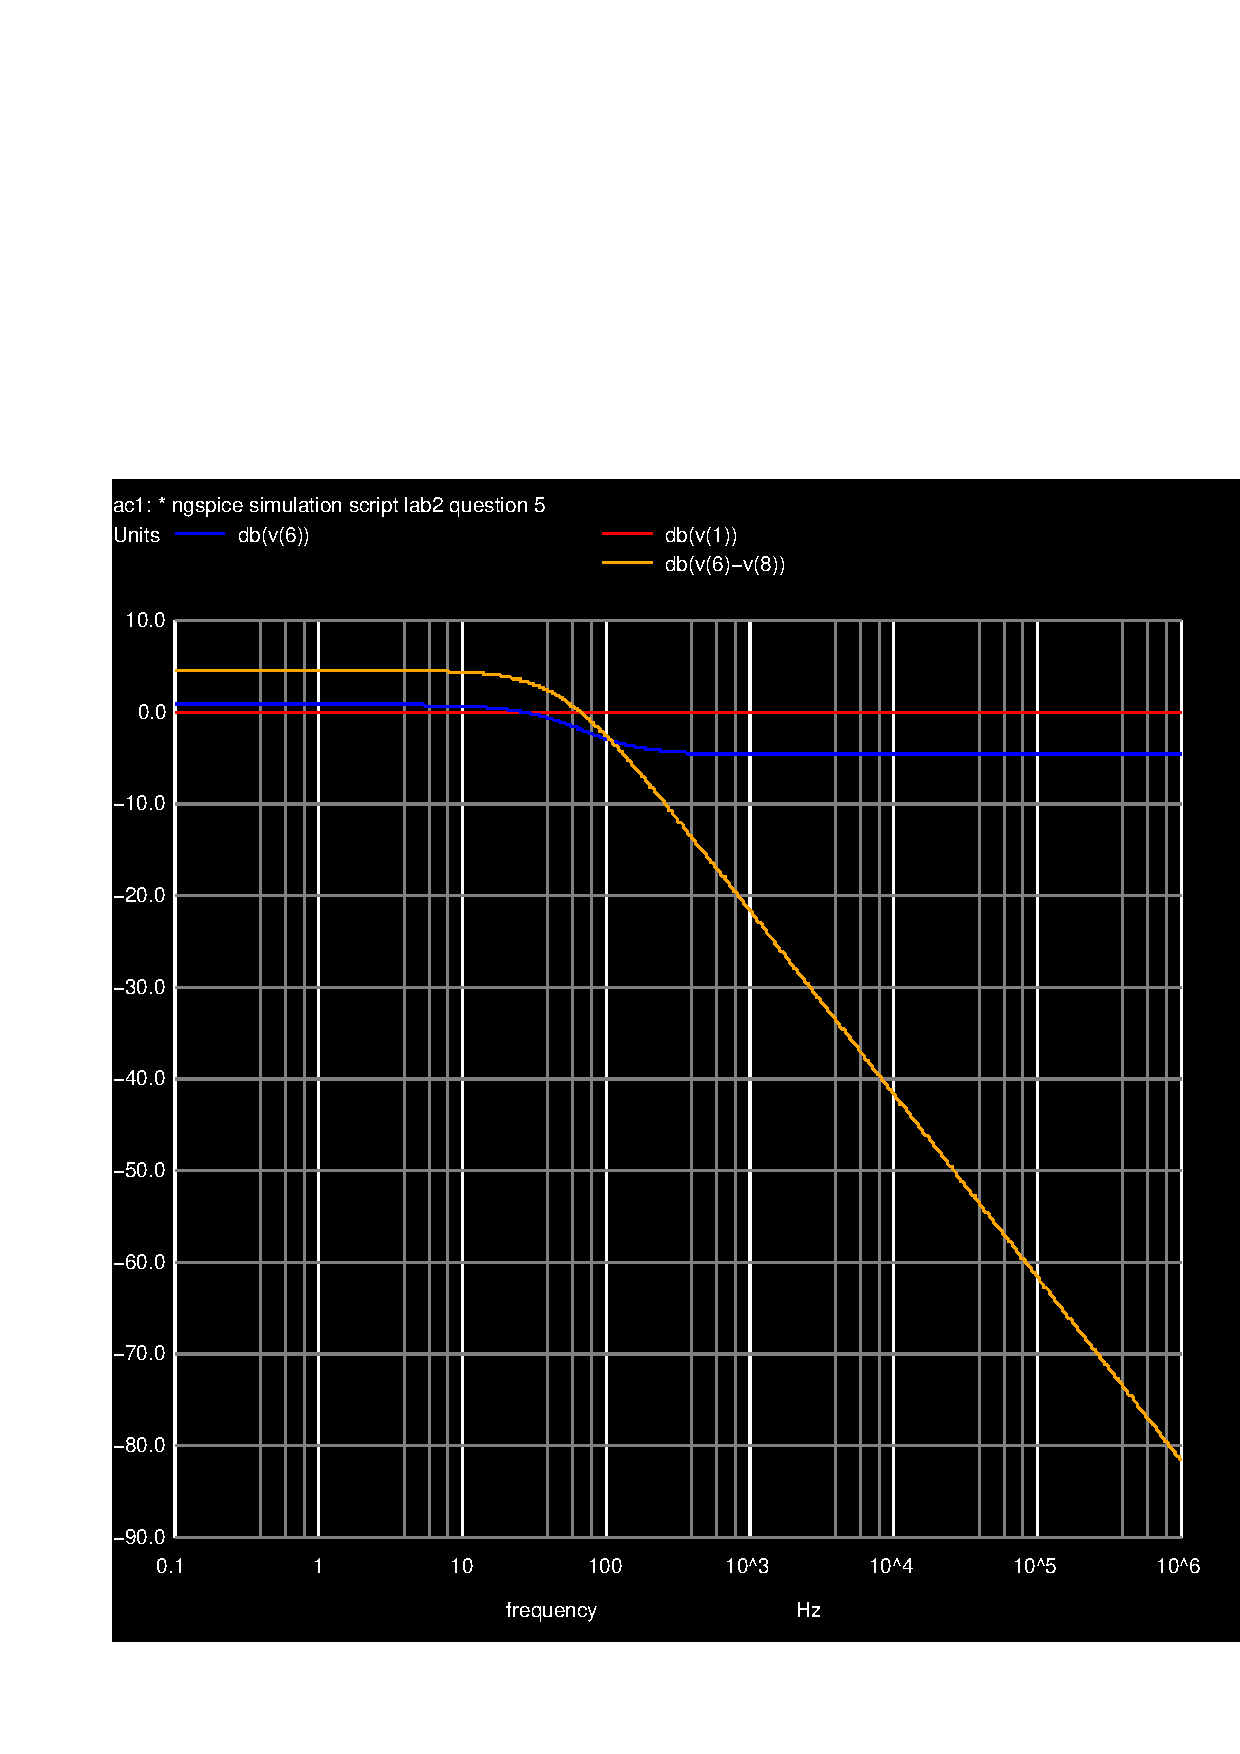
\includegraphics[width=0.9\linewidth]{sim5_db.pdf}
%\caption{Magnitude Response (in decibels)}
%\label{fig:sim5_db}
%\end{figure}

\subsubsection{Frequency Response- Phase}

\begin{figure}[ht] \centering
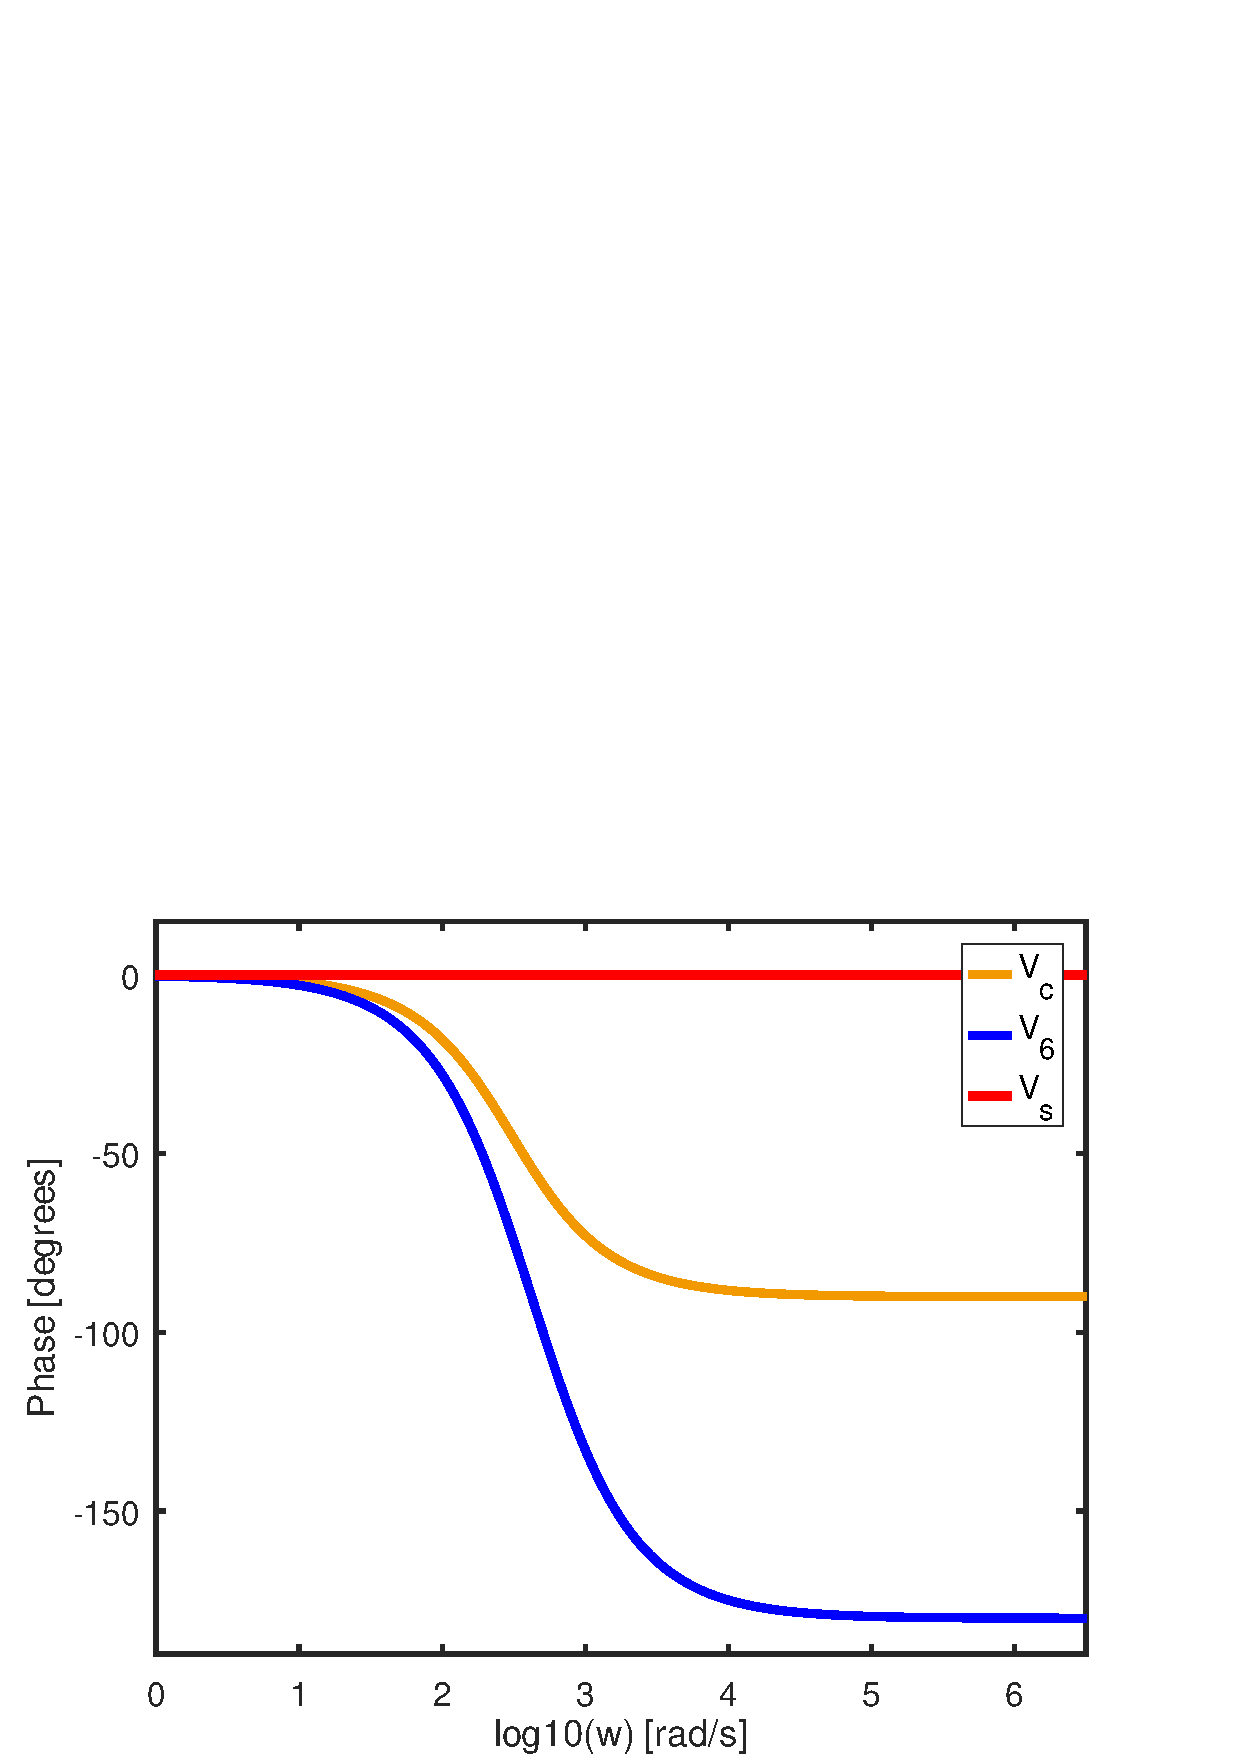
\includegraphics[width=0.9\linewidth]{part6_ang.pdf}
\caption{Circuit analysed.}
\label{RC Circuit.}
\end{figure}

%\begin{figure}[ht] \centering
%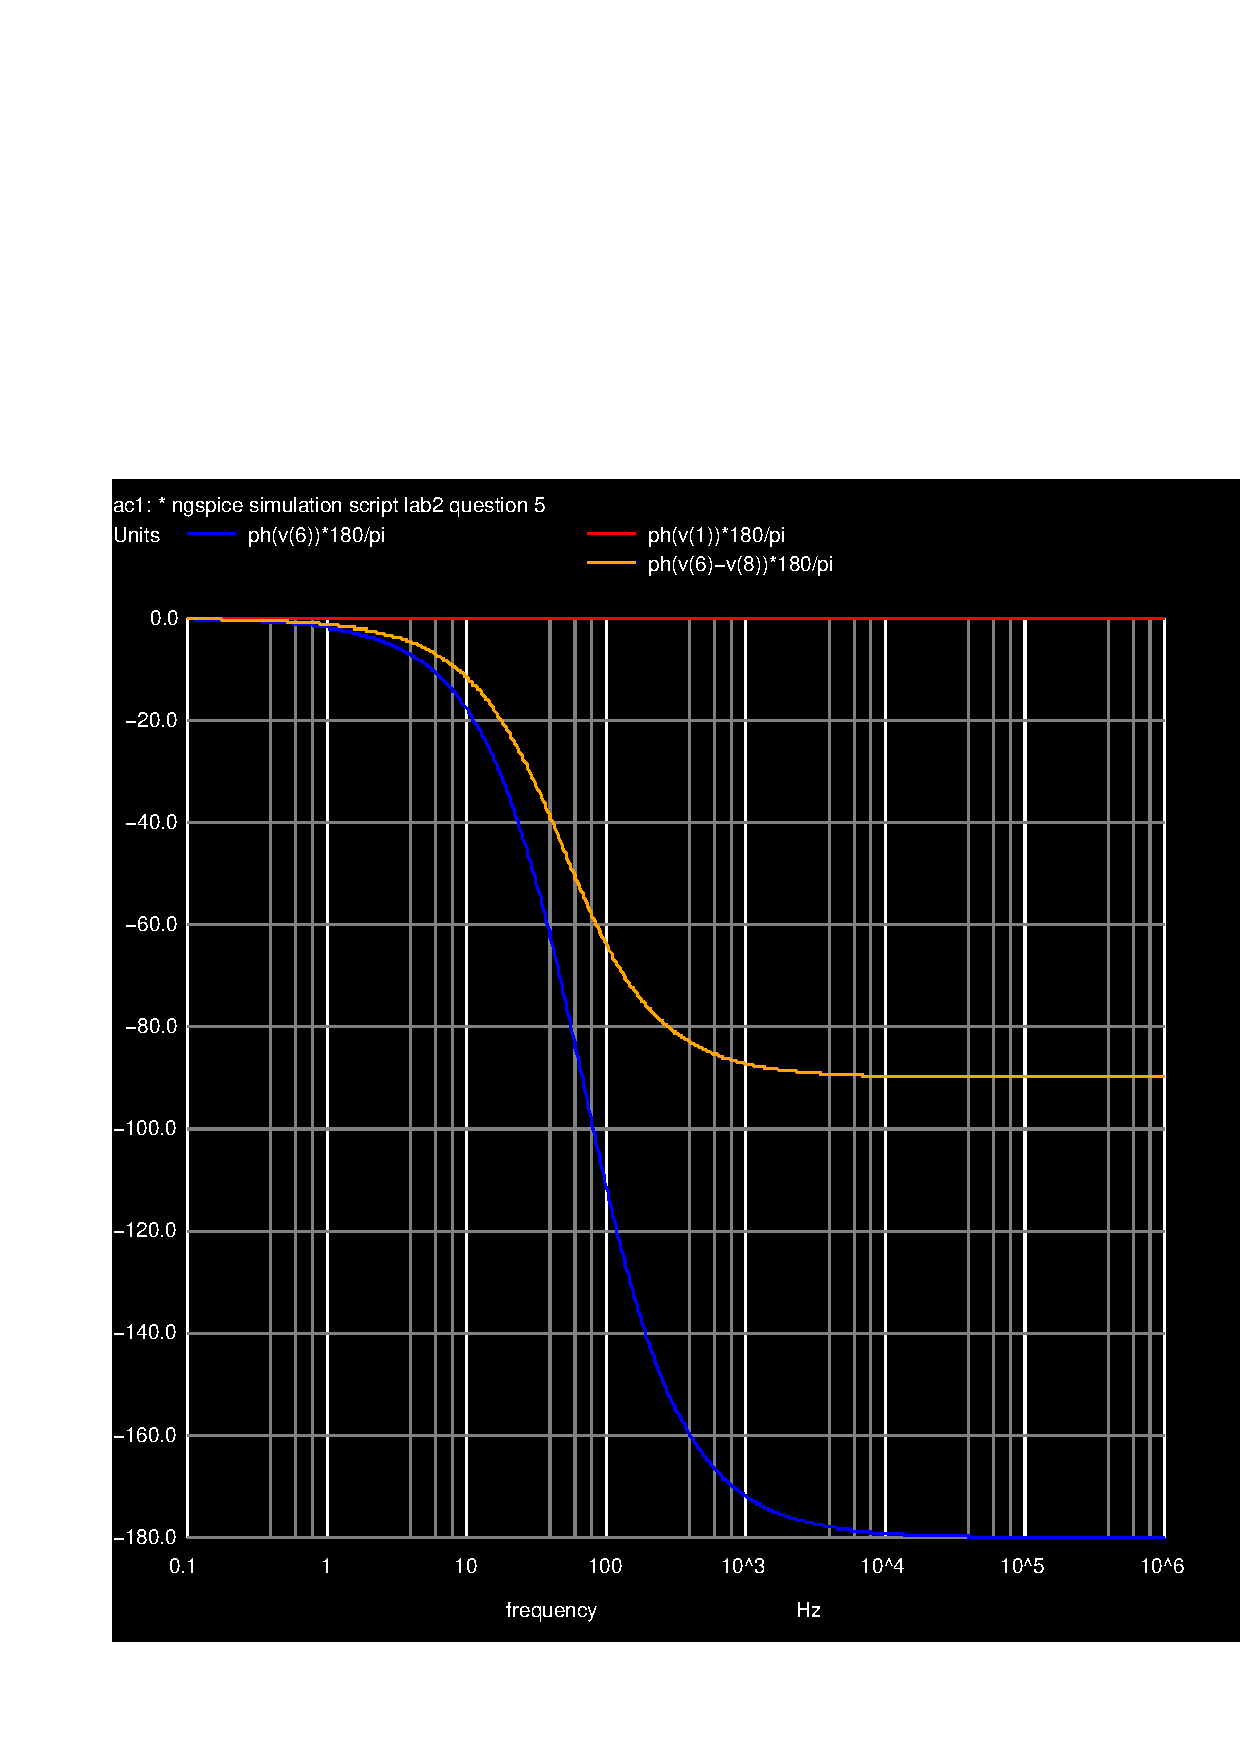
\includegraphics[width=0.9\linewidth]{sim5_ph.pdf}
%\caption{Phase Response (in degrees)}
%\label{fig:sim5_ph}
%\end{figure}

















\newpage

\pagebreak
\section{Conclusion}
\label{conclusion}

\par It was agreed by the members of the group that the main goal of the task proposed was achieved. As presented, both theoretical and simulation results(obtained using Octave tools and ngpsice simulator, in all its variants(operating, transient and frequency), respectively) matched, reaching total accuracy. Despite the initial belief that the considerable number of components of the circuit, and the number of steps needed to get to the final answer(the total solution),  could cause some disparity in the results, such did not happened.
\par To conclude, the model used can then be validated

\newpage

%\cleardoublepage

% ----------------------------------------------------------------------
%  Bibliography
% ----------------------------------------------------------------------
%\addcontentsline{toc}{section}{\bibname}
%\bibliographystyle{abbrvunsrtnat} % <<<<< SELECT IF USING REFERENCES BY NUMBER (CITATION ORDER)
%\bibliography{../../../BIBfile.bib}

% ----------------------------------------------------------------------
\end{document}
% ----------------------------------------------------------------------
